%
% Proyecto Numeros Primos y Criptografía
%
%  Jovenes a la Investigación 2021-2022
%
%  Editores: Roberto Méndez Méndez
%            Mora Itzel 
%
%  Última fecha de edición: 22 - Ene -22

\documentclass[10pt,letterpaper]{article}
\usepackage[utf8]{inputenc}
\usepackage[spanish]{babel}


\usepackage{dirtytalk} 

\usepackage{amsthm, mathtools, amsmath, amsfonts,amssymb}

\usepackage[left=2.5cm,right=2.5cm,top=2cm,bottom=1.5cm]{geometry}

%
%  Para los marcos de teoremas, ejemplos,
%					y definiciones.
% 
%  \begin{D1ejemplo}[-algún texto].
%
%  \end{D1ejemplo}

%  Editor: Roberto Méndez Méndez
%  Última edición: Agosto 2015
%        --   2-Noviembere-2018   (hay otra mejor) --
%           15-Abr-2020
%          11-Oct-2021  
%  Nombre anterior: Diseno_TeoDefEjem.tex


\usepackage[shortlabels]{enumitem}




\usepackage{tikz}
%\usetikzlibrary{tikzmark} NUNCA SE UTILIZA
%\usepackage{tkz-tab}% EN DESHUSO
\usetikzlibrary{matrix,arrows, positioning,shadows,shadings,backgrounds,
calc}

\usepackage{tcolorbox, empheq, xparse}%
\tcbuselibrary{skins,breakable,listings,theorems}


%   FORMATO TEOREMAS 

\definecolor{colordominanteD}{RGB}{74,0,148}

\newcounter{tcbteo}[section] % Contador
 %\renewcommand{\thetcbteo}{\thesection.\arabic{tcbteo}}% Formato 1.1,1.2
\renewcommand{\thetcbteo}{\arabic{tcbteo})}


% Estilo "nodoTeorema" para nodos
\tikzset{nodoTeorema/.style={%
rectangle, top color=gray!5, bottom color=gray!5,
inner sep=1mm,anchor=west,font=\small\bf\sffamily}
}
% Caja de entorno
\newtcolorbox{cajaTeorema}[3][]{%
% Opciones generales
arc=0mm,breakable,enhanced,colback=gray!5,boxrule=0pt,top=7mm,
drop fuzzy shadow, fontupper=\normalsize,
% label
step and label={tcbteo}{#3},
interior style={color=yellow!10!white},
overlay unbroken= {%
% Borde superior grueso.
% "--+(0pt,3pt)" significa: 3pt hacia arriba desde la posición anterior
\draw[colordominanteD,line width =2.5cm]
([xshift=1.25cm, yshift=0cm]frame.north west)--+(0pt,3pt);
% Borde superior 1
\draw[color=colordominanteD,line width =0.2pt]
(frame.north west)--([xshift=0pt]frame.north east);
% Caja Teorema-contador
\node[nodoTeorema](tituloteo)
at ([xshift=0.2cm, yshift=-4mm]frame.north west)
{\textbf{\color{colordominanteD} Teorema \thetcbteo \;#2}};
},
overlay first = {
% Borde superior grueso
\draw[colordominanteD,line width =2.5cm]
([xshift=1.25cm, yshift=0cm]frame.north west)--+(0pt,3pt);
% Borde superior 1
\draw[color=colordominanteD,line width =0.2pt]
(frame.north west)--([xshift=0pt]frame.north east);
% Caja Teorema-contador
\node[nodoTeorema](tituloteo)
at ([xshift=0.2cm, yshift=-4mm]frame.north west)
{\textbf{\color{colordominanteD} Teorema \thetcbteo \;#2}};
}, %First
% Nada que mantener en los cambios de página
overlay middle = { },
overlay last = { }
#1}

%- Uso \begin{teorema}... o \begin{teorema}[de tal] o \begin{teorema}[][ref]
\NewDocumentEnvironment{teoremaf2}{O{} O{} O{}}{
\bigskip\begin{cajaTeorema}{#1}{#2}%
#3
}{\end{cajaTeorema}\bigskip } 
%%%%%%%%%%%%%%%%% FIN FORMATO TEOREMA


%%%%%%%%%%%    FORMATO EJEMPLO

\newcounter{tcbejem}[section]
% \renewcommand{\thetcbejem}{\thesection.\arabic{tcbejem}} 
\renewcommand{\thetcbejem}{\arabic{tcbejem})}

\definecolor{colordominanteEj}{RGB}{34,159,159}

\tikzset{
    wnodeTeorema/.style={%
         rectangle,  top color=gray!5, bottom color=gray!5,
         inner sep=1mm,anchor=west,font=\small\bf\sffamily},
   wnodeminimo/.style={%
         rectangle,  top color=white, bottom color=white,
         text=azulF,inner sep=1mm,anchor=west,font=\small\bf\sffamily}      
}

% % Ejemplo---------------------------------------------------
\newtcolorbox{wwejemplo}[3][]{%
arc=0mm,breakable,enhanced,colback=gray!5,boxrule=0pt,
top=6mm,fontupper=\normalsize,step and label={tcbejem}{#3},
interior style={color=blue!3!white},
overlay unbroken  = {
%borde
\draw[color=gray!20,line width=0.2pt] (frame.north west)
  --([xshift=0pt]frame.north east)
  --([xshift=0pt]frame.south east);
%  --([xshift=0pt]frame.south west)--(frame.north west);
%barra vertical
\draw[color=colordominanteEj,line width=3pt] ([xshift=2pt] frame.north west)--([xshift=2pt] frame.south west);          
%Caja de Título: defi --
\node[wnodeTeorema](titulodefi) at ([xshift=4.5pt, yshift=-3mm]frame.north west)
{\textbf{Ejemplo \thetcbejem \;#2}};
                }, %overlay
overlay first  = {
%borde
\draw[color=gray!20,line width=0.2pt] (frame.north west)
  --([xshift=0pt]frame.north east)
  --([xshift=0pt]frame.south east);
%  --([xshift=0pt]frame.south west)--(frame.north west);
%barra vertical
\draw[color=colordominanteEj,line width=3pt] ([xshift=2pt] frame.north west)--([xshift=2pt] frame.south west);          
%Caja de Título: defi --
\node[wnodeTeorema](titulodefi) at ([xshift=4.5pt, yshift=-3mm]frame.north west)
{\textbf{Ejemplo \thetcbejem \;#2}};
                }, %overlay
% Mantener borde en cambio de página
overlay last    = {
%borde
\draw[color=gray!20,line width=0.2pt] (frame.north west)
  --([xshift=0pt]frame.north east)
  --([xshift=0pt]frame.south east);
%  --([xshift=0pt]frame.south west)--(frame.north west);
%barra vertical
\draw[color=colordominanteEj,line width=3pt] ([xshift=2pt] frame.north west)--([xshift=2pt] frame.south west);}
#1}
%-
\NewDocumentEnvironment{ejemplof2}{O{} O{} O{}}{\smallskip\begin{wwejemplo}{#1}{#2}%
 #3}{\end{wwejemplo}\smallskip }
 
% %FIN EJEMPLO ----------------------

%%%%%%%%%%%    FORMATO DEFINICION
\newcounter{tcbdefi}[section]
%\renewcommand{\thetcbdefi}{\thesection.\arabic{tcbdefi}}
\renewcommand{\thetcbdefi}{\arabic{tcbdefi})}

\definecolor{colordominante}{RGB}{243,102,25}

\tikzset{
    wnodeTeorema/.style={%
         rectangle,  top color=gray!5, bottom color=gray!5,
         inner sep=1mm,anchor=west,font=\small\bf\sffamily},
   wnodeminimo/.style={%
         rectangle,  top color=white, bottom color=white,
         text=azulF,inner sep=1mm,anchor=west,font=\small\bf\sffamily}      
}

% % Definición---------------------------------------------------
\newtcolorbox{wwdefinicion}[3][]{%
arc=0mm,breakable,enhanced,colback=gray!5,boxrule=0pt,
top=6mm,fontupper=\normalsize,step and label={tcbdefi}{#3},
interior style={color=blue!5!white},
overlay unbroken  = {
%borde
\draw[color=gray!20,line width=0.2pt] (frame.north west)
  --([xshift=0pt]frame.north east)
  --([xshift=0pt]frame.south east);
%  --([xshift=0pt]frame.south west)--(frame.north west);
%barra vertical
\draw[color=colordominante,line width=3pt] ([xshift=2pt] frame.north west)--([xshift=2pt] frame.south west);          
%Caja de Título: defi --
\node[wnodeTeorema](titulodefi) at ([xshift=4.5pt, yshift=-3mm]frame.north west)
{\textbf{Definición \thetcbdefi \;#2}};
                }, %overlay
overlay first  = {
%borde
\draw[color=gray!20,line width=0.2pt] (frame.north west)
  --([xshift=0pt]frame.north east)
  --([xshift=0pt]frame.south east);
%  --([xshift=0pt]frame.south west)--(frame.north west);
%barra vertical
\draw[color=colordominante,line width=3pt] ([xshift=2pt] frame.north west)--([xshift=2pt] frame.south west);          
%Caja de Título: defi --
\node[wnodeTeorema](titulodefi) at ([xshift=4.5pt, yshift=-3mm]frame.north west)
{\textbf{Definición \thetcbdefi \;#2}};
                }, %overlay
% Mantener borde en cambio de página
overlay last    = {
%borde
\draw[color=gray!20,line width=0.2pt] (frame.north west)
  --([xshift=0pt]frame.north east)
  --([xshift=0pt]frame.south east);
%  --([xshift=0pt]frame.south west)--(frame.north west);
%barra vertical
\draw[color=colordominante,line width=3pt] ([xshift=2pt] frame.north west)--([xshift=2pt] frame.south west);}
#1}
%-
\NewDocumentEnvironment{definicionf2}{O{} O{} O{}}{\smallskip\begin{wwdefinicion}{#1}{#2}%
 #3}{\end{wwdefinicion}\smallskip }
% %DEFINICION----------------------





\spanishdecimal{.}  % punto decimal 


\title{Números primos y criptografía}
\author{Cortes Mora Itzel Jesabel   \\Ordaz Rodríguez Iván \\ Asesor: Roberto Méndez Méndez}

\date{September 2021}

\begin{document}
	
	\maketitle
	\section*{Introducción}
	El antecedente del estudio de los número primos  se remonta a  Eratóstenes.
	
	
	
	\section{Algo de información}
	
	\begin{teoremaf2}
		El divisor primo más pequeño de un número compuesto n es menor que o igual a $\lfloor \sqrt{n} \rfloor$ 
		
	\end{teoremaf2}
	
	
	\section{Datos preliminares}
	\begin{definicionf2}[Función Eit(x)]
		Es la función que da 1 si $x \in \mathbb{N}$ y 0 en otro caso, es decir
		\begin{align}
			Eit(x)&=\begin{cases} 
				0 & \text{ si }x\in \mathbb{R}\backslash \mathbb{N}\\
				1 & \text{ si }x\in \mathbb{N}
			\end{cases} 
		\end{align}
	\end{definicionf2}
  La función \textit{Eit} se usará para anular los números no primos y contar solo números primos en un conjunto.


Características de la función \textit{Eit}:
\begin{enumerate}
	\item No es distributiva.
	\begin{equation*}
		Eit(Eit(a) + Eit(b)) \neq 	Eit(Eit(a)) + Eit(Eit(b)) 
	\end{equation*}
\end{enumerate}

\begin{definicionf2}[Función\textit{ E(A)}]
	Esta función regresa el número de naturales positivos ($\mathbb{N}^{+}$) en un conjunto \textit{A} 
	\begin{equation}
		E(A) = |\{ x \,|\, x \in A \text{ y } x \in \mathbb{N}^+ \}|
	\end{equation}
	donde $A \subset \mathbb{R}$ y $|A| = m$.
\end{definicionf2}
La función $E$ se define en términos de la función $Eit$ y se expresa como
\begin{equation}
	E(A) = \sum_{x \in A} \mathit{Eit}(x)
\end{equation}

\begin{definicionf2}[Función C]
	\begin{equation}
		C=\sum_{i=1}^{i_f} Eit\left(\sum_{j=8}^{j_f}Eit(m(i,j))\right)
	\end{equation}
\end{definicionf2}
	
	La suma de la fórmula anterior queda como:
	\begin{align*} 
		Eit\left(\sum_{j=8}^{j_f}Eit(m(1,j))\right)+&Eit\left(\sum_{j=8}^{j_f}Eit(m(2,j))\right)\\
		+&Eit\left(\sum_{j=8}^{j_f}Eit(m(3,j))\right)+\dots+Eit\left(\sum_{j=8}^{j_f}Eit(m(i_f,j))\right) 
	\end{align*}

	\begin{teoremaf2}[Definición de \textit{C(x)}] 
	Si $4 \leq x < 26$
	\begin{equation*}
		C(x) = 0
	\end{equation*}
	Si $x \geq 26 $, entonces
	\begin{equation*}
		C(x)	= \sum_{i = 0}^{i_f(x)} Eit\left( \sum_{j = 0}^{j_f(x)} Eit \left(\frac{4j - (-1)^j +  (2i + 1)(-1)^{i + j} + (2i - 1)(-1)^{i} - 12i^2 + 5}{12i + 6 -2 (-1)^i}\right) \right)		 
	\end{equation*}
	donde
	\begin{equation*}
		j_f(x) = \left\lceil \frac{1}{2}\left\lfloor \frac{2x + (-1)^x - 7}{3}\right\rfloor\right\rceil
	\end{equation*}	
	\begin{equation*}
		i_f(x) = \left\lceil  \frac{-1  + \sqrt{1 + 3(j_f(x))}	}{3}\right\rceil
	\end{equation*}	
\end{teoremaf2}

\begin{definicionf2}[Función $\pi(n)$ ]
La función $\pi(n)$ es definida como 
\begin{equation}
	\pi(x)   = |\left\lbrace p \in \mathbb{P} \, | \, p < x \,,\, x\in \mathbb{N} \; y \; x > 3 \right\rbrace  |
\end{equation}
es decir $\pi(x)$ es el número de primos menores  a $x$.
\end{definicionf2}
 
 \begin{teoremaf2}
 	La expresión que me da el valor de $\pi(x)$ es 
 	\begin{equation}
 		\pi(x)   = \left\lceil \frac{1}{2}\left\lfloor \frac{2x + (-1)^x - 6C(n) + 5}{3}\right\rfloor\right\rceil
 	\end{equation}
 \end{teoremaf2}	  
	\begin{proof}
		\begin{enumerate}
			\item Tomamos el triángulo rectángulo de catetos 1 y \textit{h} e hipotenusa \textit{p} tal que $p \in \mathbb{P}$ el conjunto de números primos
			% TODO: \usepackage{graphicx} required
			\begin{figure}[th!]
				\centering
				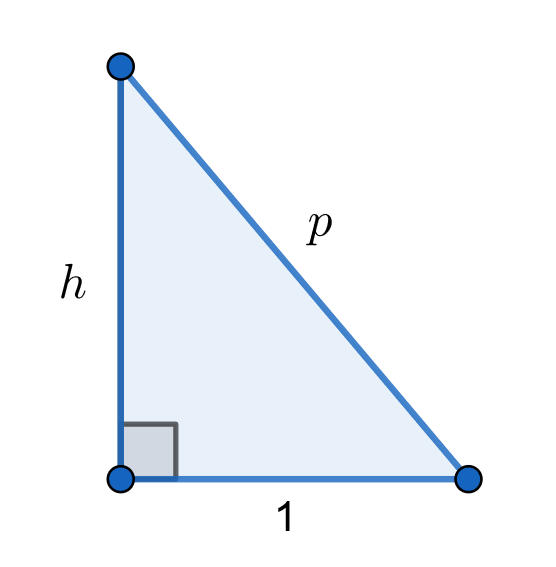
\includegraphics[scale = .7]{Imagenes/ContadorNumerosPrimos}
				\caption{Triángulo equilátero de catetos 1 y h, e hipotenusa p}
				\label{fig:contadornumerosprimos}
			\end{figure}
		luego entonces 
		\begin{equation}
			h^2 = p^2 - 1 \hspace{5mm} p > 3
		\end{equation}
			De manera experimental se construyó otra  ecuación  $k$, tal que
			\begin{equation*}
				k^{2} = \frac{-(3 + 6i)(-1)^i + 18i^2 + 18i + 3}{2} \hspace{5mm} i \geq 1
			\end{equation*}
		Igualando ambas las ecuaciones 
		\begin{equation*}
			p^2 - 1 = \frac{-(3 + 6i)(-1)^i + 18i^2 + 18i + 3}{2}
		\end{equation*}	
			se llega a que 
			\begin{equation} \label{ec:primosP_1}
				p = 
				\frac{-(-1)^i + 6i + 3}{2} \hspace{5mm} i \geq 1 
			\end{equation}
		En este caso la nueva ecuación para $p$ adolece que para una serie de valores $i$, $p$ no será primo (Vea tabla de Excel). De manera forma el dominio de la ecuación debería ser $D(h^2) \cap D(k^2)$.
		Denominaremos a este conjunto de valores donde $p$ no es primo  como $j$, es decir
		\begin{equation}
			j = \{i \in D(k^2) \, | \, p(i) \notin \mathbb{P} \}
		\end{equation}
		Algunos de estos números son $j = \{8, 11, 16,18, 21,25,28, 31, 38, 41, ... \}$
		\end{enumerate}
	La primera posición que llamare $j_{ini(p)}$ donde aparece el primer múltiplo de un primo (p > 3) no repetido, esta dada por la expresión
	\begin{equation}
		j_{ini(p)} = \frac{p^2 - 1}{3}
	\end{equation}
	al tener la posición inicial se encuentra una regularidad en la forma en que vuelven a presentarse los múltiplos de dicho primo $p$
   \begin{ejemplof2}[Caso p = 11]
   		Usando el programa en R notamos que las posiciones onde 11 tiene múltiplos son
   		\begin{equation}
   			j_{p = 11} = \{3,    18,    25,    40,    47,    62,    69,    84,    91 ,  106,   113, \ldots \}
   		\end{equation}
   	Entonces notamos que las posiciones de los múltiplas guardan una regularidad 
   	\begin{align*}
   		18 - 3 &= 15 \\
   	25  - 18 &= 7 \\
   	40 - 25 &= 15 \\
   	47 - 40 &= 7 \\
   			&\colon
   	\end{align*}
Si denominamos A = 7 y B = 15
\begin{align*}
	j_1 &  =  j_{ini(p)} + 0A + 0B\\
	j_2 & =  j_{ini(p)} + 1(A  + B) - B  \\
	j_3 & =  j_{ini(p)} + 1(A + B) + 0B \\
	j_4 &=   j_{ini(p)} + 2(A + B) - B \\
	j_5 &=  j_{ini(p)}  + 2(A + B) + 0B  \\
	&\vdots 
\end{align*}
   	\end{ejemplof2}
  Probando con diversos números primos,  una posible forma general que se encuentra es
  \begin{equation}
  	j_m = j_{ini(p)} + \varphi(m)(A + B) + \mu(m) B
  \end{equation}
con $m \in \mathbb{N}^+$ y donde  se cumple 
\begin{equation*}
	\mu(m) = \begin{cases*}
		0 & \text{ si } $m$ impar \\
		-1 & \text{ si } $m$ par 
	\end{cases*}
\end{equation*}´
y 
\begin{equation*}
	\varphi(m) = \begin{cases*}
		\frac{m}{2} & \text{ si } $m$ par \\
		\frac{m - 1}{2} & \text{ si } $m$ impar 
	\end{cases*}
\end{equation*}
las dos series son muy conocidas y tienen la forma
\begin{align}
	\mu(m) &= \frac{1}{2}\left(-(-1)^m - 1 \right) \\
	\varphi(m) &= \frac{1}{4}\left( 2m + (-1)^m - 1 \right)  
\end{align}
  Ahora obtendremos los valores de \textit{A+B} y\textit{ B} en términos de los parámetro $i$ y $p$.\\
  De la tabla que
  \begin{equation}
  	A + B = 2p
  \end{equation}
mucho más complicada es ver que
\begin{equation}
	B = -(-1)^i[-(-1)^ip + i + 0.5 - 0.5(-1)^i] 
\end{equation}
 Con los valores obtenidos par A, B $\varphi$ y $\mu$ obtenemos una expresión para el término general de la sucesión $j_m$, la cual queda dada como
 
 \begin{equation} \label{ec:j_emesimo_elemento}
 \begin{split}
 	j_m  =  \frac{p^2 - 1}{3} &+ \frac{1}{4}\left( 2m + (-1)^m - 1 \right)2p  \\
 	&+  \frac{1}{2}\left(-(-1)^m - 1 \right)\left(-(-1)^i\left[-(-1)^ip + i + 0.5 - 0.5(-1)^i\right]\right)
 \end{split}
 \end{equation}


Ahora vamos a encontrar los limites de las sumas para C(x). \\
Nuevamente hacemos otra suposición para $p$
\begin{equation*}
	p =  x + (0.5 + (0.5)(-1)^x) \hspace{5mm} x > 3
\end{equation*}
donde $ x > 3$ y $x \in \mathbb{N}$. Note que esto hace que $p$ siempre sea impar, se toma $i = j_f  + 1$ y se igual con la ecuación (\ref{ec:primosP_1})
\begin{equation*}
x + (0.5 + (-0.5)^x) = \frac{-(-1)^{j_f  +1} + 6(j_f  + 1) + 3}{2} \hspace{5mm}
\end{equation*}
despejando $j_f$  
\begin{equation*}
	j_f = \frac{2x + 1 + (-1)^x +(-1)^{j_f  +1} - 9}{6} 
\end{equation*}
y obteniendo su valor superior máximo( $(-1)^{j_f  +1} = 1$)
\begin{equation*}
	j_f = \frac{2x  + (-1)^x  - 7}{6} 
\end{equation*}

\noindent Para obtener el $i$ final que denotaremos $i_f$, en la ecuación (\ref{ec:j_emesimo_elemento}) sustituiremos $m = 1$, $i -> i_f$ y cambiaremos $p$ por la expresión dada en la ec. (\ref{ec:primosP_1}), obteniendo
\begin{align*}
	j_f &= \frac{\left(\dfrac{-(-1)^i + 6i + 3}{2}\right)^2 - 1 }{3} \\
	&= \frac{6i_f^2 - (1 + 2i_f)(-1)^{i_f} + 6i_f + 1}{2}
\end{align*} 
como busco el máximo $i_f$ , entonces este debe ser par, por lo cual
\begin{align*}
	j_f &=\frac{6i_f^2 - 4i_f }{2}\\
	   &= 3i_f^2 - 2i_f \\
	   &= 3\left(i_f^2 + \frac{2}{3}i_f + \frac{1}{9}\right) - \frac{1}{3} \\ 
	   &=\frac{ 9\left(i_f +  \frac{1}{3}\right)^2 - 1 }{3} \\ 
\end{align*}
así
\begin{equation}
	i_f = \frac{\sqrt{1 + 3i_f} - 1}{3}
\end{equation}


Ahora si procedemos a formular una expresión para C(x), donde C(x) obtiene  la diferencia entre la cantidad de valores obtenidos por $h^2$ y $k^2$, o dicho de manera más práctica, obtiene el número de números compuestos menores a \textit{x}.  

Primero despejamos \textit{m},  el valor m de  , para cada valor de i
deberá indicar si ha salido decimal o entero. En caso de salir 
un número entero, significa con ese valor de j existe un número 
no primo en , y debe contar; caso contrario, si sale un número 
con parte decimal con ese valor de j sale un número primo en 
(\ref{ec:primosP_1}), y debe anularse.
\\

Pero para encontrar la cantidad de valores de i que reemplazando 
en (\ref{ec:primosP_1}) sale un número compuesto, se necesita saber aún hasta 
que número se reemplazará de i en , para luego contar cuantos 
números compuestos hay. Recordando, que j es una sucesión que 
empieza en el número 8, y la sucesión i empieza en 1; se 
requiere un límite para cada sucesión que se encontrará en el 
conjunto  .


Ahora obtengamos finalmente $\pi(x)$ pero esto es inmediato
pues
\begin{align*}
	\pi(x) = j_f - C(x) + 2
\end{align*}
de donde
		
\end{proof}	
\section{Algoritmo RSA}
	\subsection{Cifrado por llave secreta}
	El algoritmo RSA fue el primer algoritmo de cifrado de clave pública del mundo, y aunque con modificaciones a resistido la prueba del tiempo notablemente bien. Este esquema de cifrado asimétrico fue creado en 1977 por  Ronald Rivest, Adi Shamir and Leonard
	Adleman , de ahí el nombre RSA acrónimo de las iniciales de  sus apellidos.
	Este tipo de cifrado se basa en el principio de Kerckhoffs el cual establece lo siguiente:\\ 
	\say {La seguridad no debe ser el resultado de mantener en secreto el mecanismo de cifrado, sino más bien el resultado de conservar privada una parte cambiable del mecanismo de encriptación, -llamada llave secreta-}.\\
	 Algunas de sus posteriores modificaciones  han sido las siguientes:

	\begin{enumerate}
		\item En 1995, Kuwakado, Koyama y Tsuruoka presentaron un nuevo esquema de tipo RSA basado en curvas cúbicas singulares 
		\begin{equation*}
			y^2 \mod x^3 + bx^2 \qquad (mod \, N)
		\end{equation*}
		\noindent donde $N = pq$ es un módulo RSA. 
		\item  En 2002, Elkamchouchi, Elshenawy y Shaban introdujeron una extensión del esquema RSA al campo de enteros Gaussianos, usando un módulo $N = PQ$
		donde \textit{P} y \textit{Q} son primos Gaussianos tal que $p = |P|$ y $q = |Q|$
		son primos ordinarios. 
		\item En 2007, Castagnos propuso un esquema sobre ``quadratic field quotients '' con un módulo RSA, $ N = pq$
	\end{enumerate} 
 En los tres esquemas anteriores, el exponente público \textit{e} es un entero que satisface la ecuación clave \\ $ed - k(p^2 - 1)(q^2- 1) =1$. \\
 En este texto nos basaremos en la implementación clásica, la cual si bien más simple no por eso menos significativa para el aprendizaje de los elementos sustantivos en este algoritmo.
	


\begin{thebibliography}{100}
	\bibitem{PaPe} Paar \& Pelzl, (2010). Understanding Cryptography, Springer. // Cap. 7 The RSA Cryptosysmen.
	\bibitem{Sma} Smart, (2016). Cryptography Made Simple, Springer. // Chapter 15. The Naive RSA Algorithm
	\bibitem{LiSt} Liu \& Steinfeld (Eds.)(2016).Information Security and Privacy, Springer . // pág. 258 
	\bibitem{Bue} Buell (2021). Fundamentals of Criptography. // Poner ejemplo de la página 8 
\end{thebibliography}

\end{document} 


